\documentclass[11pt]{article}

% load some asm stuff -
\usepackage{amssymb}
\usepackage{amsmath}
\usepackage{amsthm}
%\usepackage{palatino,lettrine}
\usepackage{fancyhdr}
\usepackage{epsfig}
\usepackage[round,comma,sort]{natbib}
\usepackage{simplemargins}
\usepackage{setspace}
\usepackage[margin=0pt,font=small,labelfont=bf]{caption}

\bibliographystyle{plos2009}

% Set the size
%\textwidth = 6.75 in
%\textheight = 9.75 in
%\oddsidemargin = 0.0 in
%\evensidemargin = 0.0 in
%\topmargin = 0.01 in
%\headheight = 0.0 in
%\headsep = 0.25 in
%\parskip = 0.15in
\doublespace

\setallmargins{1in}

\newtheorem{example}{Example}[section]
\newtheorem{thm}{Theorem}[section]
\newtheorem{property}{Property}[section]

\theoremstyle{definition}
\newtheorem{defn}[thm]{Definition}

\makeatletter
\renewcommand\subsection{\@startsection
	{subsection}{2}{0mm}
	{-0.05in}
	{-0.5\baselineskip}
	{\normalfont\normalsize\bfseries}}
\renewcommand\subsubsection{\@startsection
	{subsubsection}{2}{0mm}
	{-0.05in}
	{-0.5\baselineskip}
	{\normalfont\normalsize\itshape}}
\renewcommand\paragraph{\@startsection
	{paragraph}{2}{0mm}
	{-0.05in}
	{-0.5\baselineskip}
	{\normalfont\normalsize\itshape}}
\makeatother
\linespread{1.2}

\fancypagestyle{proposal}{\fancyhf{}%
	\fancyhead[RO,LE]{\thepage}%
	\fancyhead[LO,RE]{ChE 525 Analysis of Well-Mixed Batch Cultures}%
	\renewcommand\headrulewidth{1pt}}
\pagestyle{proposal}

% Single space'd bib -
\setlength\bibsep{0pt}

\renewcommand{\rmdefault}{phv}\renewcommand{\sfdefault}{phv}

%\newboxedtheorem[boxcolor=black, background=gray!5,titlebackground=orange!20,titleboxcolor = black]{color_box_example}{Example}{test}

% Change the number format in the ref list -
\renewcommand{\bibnumfmt}[1]{#1.}

% Change Figure to Fig.
\renewcommand{\figurename}{Fig.}

%Joycelyn Chan, Joshua Lequieu, Michael Paull, Chidanand Balaji, Ryan Tasseff
%Our derivation follows closely the earlier development of Fredrickson \citep{Fredrickson:1976fk}.

% Begin ...
\begin{document}

%\begin{titlepage}
{\par\centering\textbf{\Large Analysis of Well-Mixed Batch Cultures using Unstructured Models}}
\vspace{0.2in}
{\par \centering \large{Jeffrey D. Varner$^{*}$}}
\vspace{0.05in}
{\par \centering \large{School of Chemical Engineering$^{*}$}}
{\par \centering \large{Purdue University, West Lafayette IN 47907}}
\vspace{0.1in}
{\par \centering \small{Copyright \copyright\ Jeffrey Varner 2016. All Rights Reserved.}}\\

%\end{titlepage}
\date{}
\thispagestyle{empty}

\setcounter{page}{1}

%material and energy balances around the different processes cells do. For example, understanding how the abundance of raw materials in a bioreactor influences
%cell growth, or the production of valuable protein or small molecule products requires a materials balances around the major components of the system.
%The production of valuable small molecule or protein products requires large connected intracellular reaction networks that produce or consume energy.
%Thus, to understand the operation of biochemical systems and ultimately to manipulate them for societal gain,

\section*{Introduction}
Batch cultures are the simplest type of liquid culture that can be run. In a batch culture, there is not flow into or from the reaction vessel.
Thus, there are no pumps or control systems to monitor and adjust flow rates, you simply fill a flask with nutrient rich broth, inoculate the flask with cells, and let the culture proceed.
While batch cultures are experimentally simple to run, they are \textit{more~complex} than continuous cultures because they are dynamic. In this lecture, we'll develop a mathematical description of
batch cultures using the general material balances, and then explore which model parameters we can be estimated with batch culture data.

\subsection*{General model equations for batch cultures.}
Let's start with the general material balances we derived previously:
\begin{eqnarray}\label{eqn-metabolite-dilution-dynamic}
	\frac{dC_{j}}{dt} &=& \sum_{s~=~1}^{\mathcal{S}}v_{s}D_{s}C_{j,s} + \left(\sum_{r~=~1}^{\mathcal{R}}\sigma_{jr}\hat{r}_{r}\right) + \left(\sum_{k~=~1}^{\mathcal{T}}\tau_{j,k}q_{k}\right)X  - \frac{C_{j}}{V}\frac{dV}{dt}\qquad j=1,2,\dots,\mathcal{M}\\
	\frac{dX}{dt} &=& \sum_{s~=~1}^{\mathcal{S}}v_{s}D_{s}X_{s}+\left(\mu - k_{d}\right)X - \frac{X}{V}\frac{dV}{dt}\\
	\frac{dV}{dt} &=& \sum_{s~=~1}^{\mathcal{S}}v_{s}\frac{\rho_{s}}{\rho}F_{s} - \frac{V}{\rho}\frac{d\rho}{dt}
\end{eqnarray}where the quantity $D_{s}$,  called a \textit{dilution~rate} (hr$^{-1}$), is given as:
\begin{equation}
	D_{s} \equiv \frac{F_{s}}{V}\qquad s=1,2,\dots,\mathcal{S}
\end{equation}The quantity $C_{j}$ denotes the concentration of the jth extracellular metabolite, $V$ denotes the working volume of the culture and $X$ denotes the cellmass.
In a batch culture, there is not flow into or from the culture vessel, thus $D_{s} = 0~\forall{s}$. Because there is no flow, there is no volume change ($dV/dt = 0$), and all the dilution terms in the material balances vanish leaving:
\begin{eqnarray}\label{eqn-metabolite-batch}
	\frac{dC_{j}}{dt} &=& \left(\sum_{r~=~1}^{\mathcal{R}}\sigma_{jr}\hat{r}_{r}\right) + \left(\sum_{k~=~1}^{\mathcal{T}}\tau_{j,k}q_{k}\right)X \qquad j=1,2,\dots,\mathcal{M}\\
	\frac{dX}{dt} &=& \left(\mu - k_{d}\right)X
\end{eqnarray}

\subsection*{Analysis of a simple batch culture.}
To better understand the dynamics of a batch culture, let's simplify the general equations by assuming a Monod growth model \citep{Legout:2010aa}, a single limiting nutrient $S$, and by neglecting product formation and maintenance utilization of substrate.
With these assumptions the general batch balances reduce to:
\begin{eqnarray}\label{eqn-metabolite-batch-simple}
	\frac{dS}{dt} &=& -\frac{1}{Y_{X/S}^{*}}\mu~X\\
	\frac{dX}{dt} &=& \left(\mu - k_{d}\right)X
\end{eqnarray}
where $\mu$ is given by:
\begin{equation}\label{eqn-monod-growth-model}
	\mu = \mu_{g}^{max}\left(\frac{S}{K_{g} + S}\right)
\end{equation}
The cellmass and substrate balances are coupled nonlinear differential equations which can be solved numerically using common packages such as MATLAB or JULIA \citep{BEKS14} (Fig. \ref{fig-batch}).
Cell mass growth occurs in three phases: lag, exponential and stationary/death phases. During the lag-phase, cells are manufacturing the proper systems internally to process the substrate.
Once this adaptation phase is complete, cells begin to process substrate as quickly as possible which leads to a phase of maximum growth called the exponential phase.
Once the substrate is exhausted, cells no longer divide, and growth stops leading to the stationary/death phase of the culture.

\begin{figure*}[!h]\centering
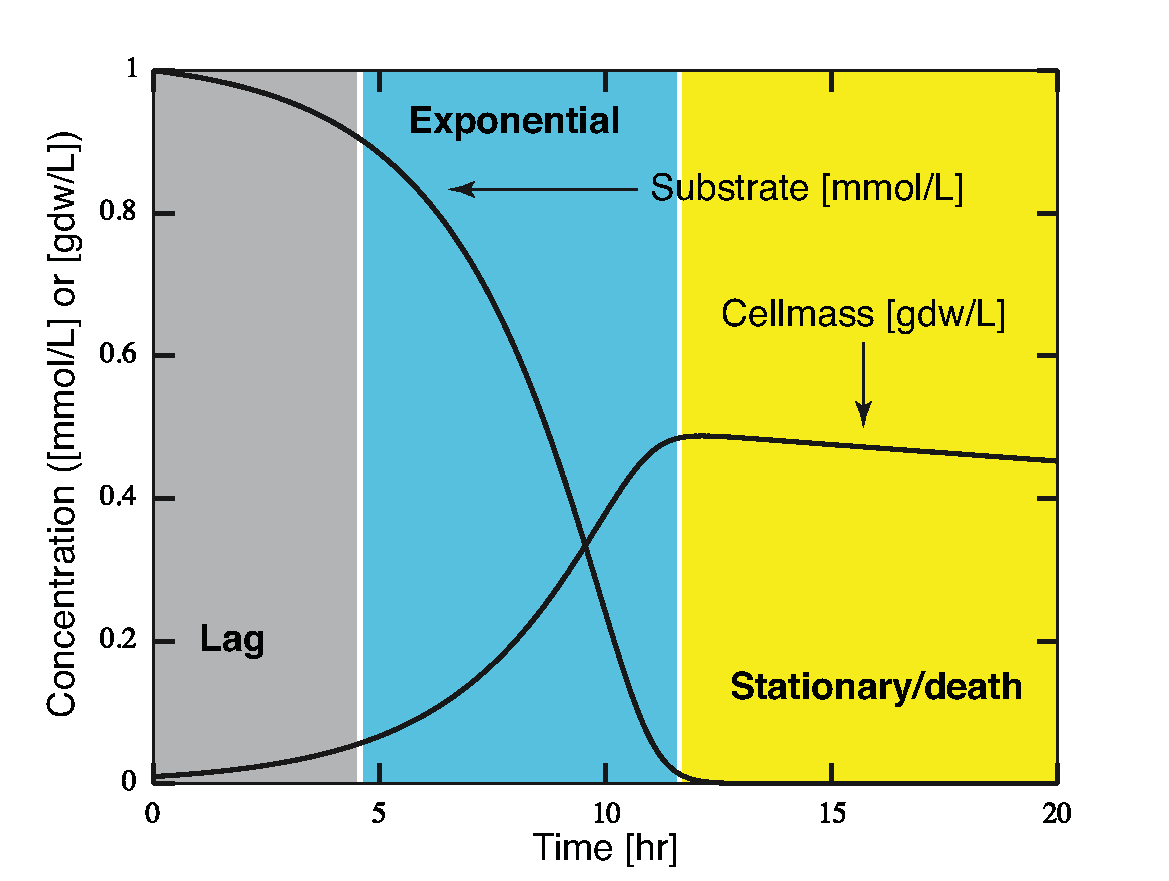
\psfig{file=figs/Batch-Final-eps-converted-to.pdf,width=0.8\textwidth}
\caption{Theoretical growth and substrate curve for cells in a well-mixed batch culture as a function of time.
The x-axis denotes time [hr] while the y-axis denotes the cellmass (X) [gdw/L] or substrate (S) [mmol/L] concentration.}\label{fig-batch}
\end{figure*}

\subsubsection{Estimation of model parameters.}
The simplified batch model equations with Monod growth kinetics have four unknown parameters; the maximum specific growth rate $\mu_{g}^{max}$, the saturation coefficient $K_{g}$, the cell death constant $k_{d}$ and the cellmass yield on substate
$Y_{X/S}^{*}$. We can use measurements of the cellmass (X) and substrate (S) to estimate these parameters.

To estimate the yield, we take the ratio of the difference between the substate and cellmass measurements at the beginning of the culture
and at the end of the exponential growth phase. Recall, the definition of the cellmass yield on substrate is given by:
\begin{equation}
	Y_{X/S} = - \frac{\Delta X}{\Delta S}
\end{equation}Expanding the differences gives:
\begin{equation}
	Y_{X/S} = -\frac{X(T) - X(0)}{S(T) - S(0)}\simeq \frac{X(T)}{S(0)}
\end{equation}where $t=T$ denotes the end of exponential phase. Note that we have not estimated $Y_{X/S}^{*}$, rather we have estimated the apparent yield. The difference between these quantities is associated with the maintenance
utilization of substrate. In out case, the true yield ($Y_{X/S}^{*}$) and the apparent yield ($Y_{X/S}$) are equal (becuase we have neglected maintenance), however this is not generally true.

The cell death rate constant can be estimated from the cellmass measurements during the stationary/death phase of the batch culture.
During this phase, $\mu = 0$, thus the cellmass balance reduces to:
\begin{equation}
	\frac{dX}{dt} \simeq -k_{d}X
\end{equation}Rearranging and expanding the derivative gives:
\begin{equation}
	-\frac{1}{X(t_{0})}\frac{X(t_1) - X(t_{-1})}{t_{1} - t_{-1}}\simeq k_{d}
\end{equation}where $t_{-1},t_{0}$ and $t_{1}$ are three sequential time points during the stationary/death phase, and $X(t_{*})$ denotes a cellmass measurement at time point $t_{*}$.

To estimate both $K_{g}$ and $\mu_{g}^{max}$ we need to make use of the growth model. We know that at \textit{anytime} during the culture the growth rate is given by Eqn \eqref{eqn-monod-growth-model}.
Thus, we can rearrange the growth model to give:
\begin{equation}\label{eqn-eqn-double-recip}
	\frac{1}{\mu} = \left(\frac{K_{g}}{\mu_{g}^{max}}\right)\frac{1}{S}+\frac{1}{\mu_{g}^{max}}
\end{equation}Eqn \eqref{eqn-eqn-double-recip} is called a \textit{double~reciprical};
we use this relationship in combination with estimates of the growth rate and substrate measurements to uniquely determine \textit{both} $K_{g}$ and $\mu_{g}^{max}$
from the slope and intercept of the double reciprocal plot (1/S versus 1/$\mu$).

A quick and dirty approximation of $\mu_{g}^{max}$ can also be obtained by estimating the growth rate during the exponential phase; during the exponential phase the culture growth rate is approximately $\mu\simeq\mu_{g}^{max}$ which reduces
the cellmass balance to:
\begin{equation}\label{eqn-expphase-batch-cellmass}
	\frac{dX}{dt} \simeq \left(\mu_{g}^{max} - k_{d}\right)X
\end{equation}Assumming that we have already estimated $k_{d}$, the only unknown in Eqn \eqref{eqn-expphase-batch-cellmass} is $\mu_{g}^{max}$:
\begin{equation}
	\frac{1}{X}\frac{dX}{dt}+k_{d} \simeq \mu_{g}^{max}
\end{equation}or
\begin{equation}
	\frac{1}{X(t_{0})}\frac{X(t_1) - X(t_{-1})}{t_{1} - t_{-1}} + k_{d} \simeq \mu_{g}^{max}
\end{equation}where $t_{-1},t_{0}$ and $t_{1}$ are three sequential time points during the exponential phase, and $X(t_{*})$ denotes a cellmass measurement at time point $t_{*}$.


\bibliography{Notes}
\end{document}
